% Figure: one RealNVP affine coupling layer.
% Teaching point: the coupling layer is invertible in closed form AND its
% block-triangular Jacobian collapses to sum_j s_theta,j(x_a), which is what
% makes exact likelihood cheap.  Design width ~168mm.
\documentclass[border=0pt]{standalone}
\usepackage{amsmath,amssymb}
% Shared visual language for the figures of the book.
% Every figure in this directory loads this file so the chapter reads as one system.
% NOTE: no blank lines are allowed inside \tikzset{...} (a blank line emits \par
% and breaks key scanning).
\NeedsTeXFormat{LaTeX2e}
\ProvidesPackage{figstyle}[2026/10/21 Figure style for Free Energy to LLMs]

\RequirePackage{tikz}
\usetikzlibrary{arrows.meta,positioning,calc,fit,shapes.geometric,shapes.misc,%
  backgrounds,matrix,decorations.pathreplacing,decorations.markings,patterns.meta}

% ---------------------------------------------------------------- palette
% Same values as book/preamble/style.tex, prefixed with F.
\definecolor{FNavy}{HTML}{14324A}
\definecolor{FTeal}{HTML}{0E7490}
\definecolor{FSky}{HTML}{E7F5F8}
\definecolor{FOrange}{HTML}{D97706}
\definecolor{FAmber}{HTML}{FFF3D6}
\definecolor{FInk}{HTML}{1F2937}
\definecolor{FSlate}{HTML}{64748B}
\definecolor{FMist}{HTML}{F5F7FA}
\definecolor{FRose}{HTML}{9F1239}
\definecolor{FRoseMist}{HTML}{FFF1F2}

% ---------------------------------------------------------------- semantics
% Teal   = probability / model / data object
% Orange = training objective, cost, or the quantity moved through the system
% Navy   = neutral structure
% Slate  = secondary label or metadata
% Rose   = failure mode, hazard, masked-out region
\tikzset{
  % Lay figures out in millimetres.  A figure designed 168mm wide is included at
  % \textwidth, so its fonts appear at exactly the size written here.
  every picture/.style={x=1mm,y=1mm,font=\small,line cap=round,line join=round},
  % ---- block styles
  nbase/.style={draw,rounded corners=1.2pt,align=center,inner sep=2.4pt,%
    minimum height=7mm,text=FInk},
  nteal/.style={nbase,draw=FTeal,fill=FSky},
  norange/.style={nbase,draw=FOrange,fill=FAmber},
  nnavy/.style={nbase,draw=FNavy,fill=white},
  nsoft/.style={nbase,draw=FSlate!55,fill=FMist},
  nrose/.style={nbase,draw=FRose,fill=FRoseMist},
  ghost/.style={draw=none,fill=none,align=center,inner sep=1pt},
  plain/.style={draw=none,fill=none,align=center,inner sep=0pt},
  % ---- arrows
  ar/.style={-{Latex[length=1.7mm,width=1.35mm]},draw=FSlate,line width=0.75pt},
  ard/.style={ar,dashed},
  arteal/.style={ar,draw=FTeal},
  arorange/.style={ar,draw=FOrange},
  arrose/.style={ar,draw=FRose},
  thickar/.style={ar,line width=1.2pt},
  % ---- text roles
  ftitle/.style={font=\large\bfseries,text=FNavy,align=center},
  ptitle/.style={font=\small\bfseries,text=FNavy,align=center},
  ptitleo/.style={font=\small\bfseries,text=FOrange,align=center},
  lbl/.style={font=\scriptsize,text=FSlate,align=center,inner sep=1pt},
  lblt/.style={lbl,text=FTeal},
  lblo/.style={lbl,text=FOrange},
  lbln/.style={lbl,text=FNavy},
  lblr/.style={lbl,text=FRose},
  sub/.style={font=\scriptsize,text=FSlate!90,align=center,inner sep=1pt},
  monob/.style={font=\ttfamily\scriptsize,text=FInk,inner sep=1pt},
  mathb/.style={font=\small,text=FInk,inner sep=1pt},
  eqn/.style={font=\scriptsize,inner sep=1.5pt,text=FInk},
  % ---- decorations
  brace/.style={decorate,decoration={brace,amplitude=2.4pt},draw=FSlate,%
    line width=0.6pt},
  bracet/.style={brace,draw=FTeal},
  braceo/.style={brace,draw=FOrange},
  axis/.style={draw=FSlate!55,line width=0.6pt},
  guide/.style={draw=FSlate!45,line width=0.5pt,dashed},
  halolabel/.style={font=\scriptsize,text=FInk,fill=white,fill opacity=0.85,%
    text opacity=1,inner sep=1.4pt,align=center},
}

% Figure title above the drawing, anchored at the figure's top-left.
\newcommand{\figtitle}[2][0]{%
  \node[ftitle,anchor=north west,outer sep=0pt] at (#1,0) {#2};}

% Rounded panel behind a subgroup of nodes.
\newcommand{\figpanel}[3][]{%
  \node[draw=FSlate!35,fill=#3,rounded corners=2pt,inner sep=2.6mm,#1] {#2};}

\endinput

\begin{document}
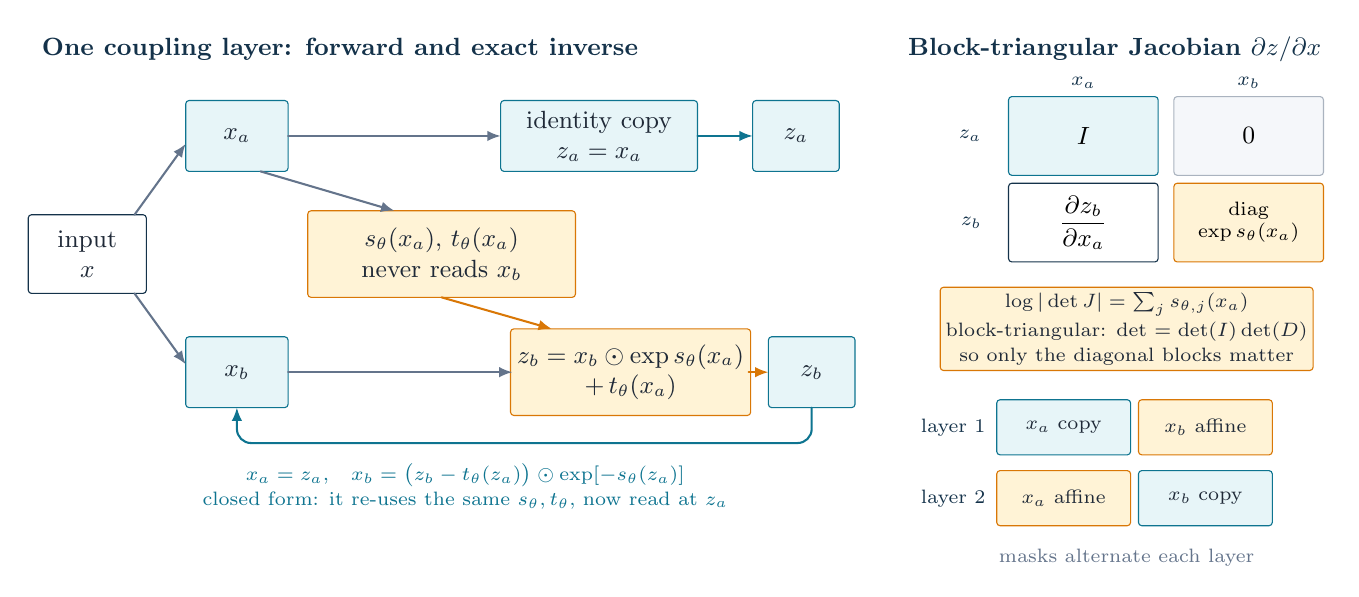
\begin{tikzpicture}
% ============================================================ panel (a) title
\node[ptitle,anchor=west] at (0,61) {One coupling layer: forward and exact inverse};

% ------------------------------------------------- forward: the two branches
\node[nnavy,minimum width=15mm,minimum height=10mm] (xin) at (7,35) {input\\$x$};
\node[nteal,minimum width=13mm,minimum height=9mm] (xa) at (26,50) {$x_a$};
\node[nteal,minimum width=13mm,minimum height=9mm] (xb) at (26,20) {$x_b$};

\node[norange,minimum width=34mm,minimum height=11mm] (net) at (52,35)
  {$s_\theta(x_a),\,t_\theta(x_a)$\\ never reads $x_b$};

\node[nteal,minimum width=25mm,minimum height=9mm] (copy) at (72,50)
  {identity copy\\$z_a=x_a$};
\node[norange,minimum width=30mm,minimum height=11mm] (aff) at (76,20)
  {$z_b=x_b\odot\exp s_\theta(x_a)$\\$+\,t_\theta(x_a)$};

\node[nteal,minimum width=11mm,minimum height=9mm] (za) at (97,50) {$z_a$};
\node[nteal,minimum width=11mm,minimum height=9mm] (zb) at (99,20) {$z_b$};

\draw[ar] (13,40)--(19.5,49);
\draw[ar] (13,30)--(19.5,21);
\draw[ar] (29,45.5)--(46,40.5);
\draw[ar] (32.5,50)--(59.5,50);
\draw[ar] (32.5,20)--(61,20);
\draw[arorange] (52,29.5)--(66,25.5);
\draw[arteal] (84.5,50)--(91.5,50);
\draw[arorange] (91,20)--(93.5,20);

% ------------------------------------- the inverse, drawn as a usable arrow
\draw[arteal,rounded corners=1.8mm] (99,15.5)--(99,11)--(26,11)--(26,15.5);
\node[lblt,align=center] at (55,5.5)
  {$x_a=z_a$,\quad $x_b=\big(z_b-t_\theta(z_a)\big)\odot\exp[-s_\theta(z_a)]$\\[1pt]
   closed form: it re-uses the same $s_\theta,t_\theta$, now read at $z_a$};

% ============================ panel (b): the block-triangular Jacobian matrix
\node[ptitle,anchor=west] at (110,61) {Block-triangular Jacobian $\partial z/\partial x$};

\node[draw=FTeal,fill=FSky,rounded corners=1.2pt,inner sep=0pt,%
      minimum width=19mm,minimum height=10mm] at (133.5,50) {$I$};
\node[draw=FSlate!55,fill=FMist,rounded corners=1.2pt,inner sep=0pt,%
      minimum width=19mm,minimum height=10mm] at (154.5,50) {$0$};
\node[draw=FNavy,fill=white,rounded corners=1.2pt,inner sep=0pt,%
      minimum width=19mm,minimum height=10mm] at (133.5,39)
  {$\dfrac{\partial z_b}{\partial x_a}$};
\node[draw=FOrange,fill=FAmber,rounded corners=1.2pt,inner sep=0pt,%
      minimum width=19mm,minimum height=10mm,align=center,font=\scriptsize]
  at (154.5,39) {$\mathrm{diag}$\\$\exp s_\theta(x_a)$};

\node[lbln,anchor=south] at (133.5,55.6) {$x_a$};
\node[lbln,anchor=south] at (154.5,55.6) {$x_b$};
\node[lbln,anchor=east] at (121,50) {$z_a$};
\node[lbln,anchor=east] at (121,39) {$z_b$};

\node[draw=FOrange,fill=FAmber,rounded corners=1.2pt,align=center,%
      inner sep=2pt,font=\scriptsize,text=FInk] at (139,25.5)
  {$\log|\det J|=\sum_j s_{\theta,j}(x_a)$\\[1pt]
   block-triangular: det $=\det(I)\det(D)$\\[1pt]
   so only the diagonal blocks matter};

% ================= panel (c): the mask alternates, so nothing stays untouched
\node[lbln,anchor=east] at (121.5,13) {layer 1};
\node[lbln,anchor=east] at (121.5,4) {layer 2};
\node[nteal,minimum width=17mm,minimum height=7mm,font=\scriptsize] at (131,13) {$x_a$ copy};
\node[norange,minimum width=17mm,minimum height=7mm,font=\scriptsize] at (149,13) {$x_b$ affine};
\node[norange,minimum width=17mm,minimum height=7mm,font=\scriptsize] at (131,4) {$x_a$ affine};
\node[nteal,minimum width=17mm,minimum height=7mm,font=\scriptsize] at (149,4) {$x_b$ copy};
\node[lbl,anchor=north] at (139,-2) {masks alternate each layer};
\end{tikzpicture}
\end{document}
